\documentclass[border=6pt]{standalone}
\usepackage{fontspec}
\usepackage[sfdefault,lining]{FiraSans}
\usepackage{pgfplots}
\usepgfplotslibrary{groupplots}
\pgfplotsset{compat=1.18}
\definecolor{tsnavy}{HTML}{1A2E4F}\definecolor{tsred}{HTML}{A6252D}\definecolor{tsink}{HTML}{1F2430}
\definecolor{tsgrey}{HTML}{5F6B7C}\definecolor{tsmuted}{HTML}{A7B2C2}\definecolor{tsline}{HTML}{D6DCE5}
\definecolor{cRepair}{HTML}{1B7F9E}\definecolor{cControl}{HTML}{C98A2B}
\definecolor{cVanOurs}{HTML}{F2C3C6}\definecolor{cVanPaper}{HTML}{8AA4CC}
\pgfplotsset{rd/.style={axis lines*=left, ymajorgrids, grid style={tsline,line width=0.4pt},
  axis line style={tsgrey,line width=0.5pt}, major tick style={draw=none},
  tick label style={font=\small,text=tsgrey,/pgf/number format/assume math mode=true}, label style={font=\small,text=tsink},
  title style={font=\bfseries\color{tsnavy}},
  legend style={draw=none,fill=none,font=\small,text=tsink,/tikz/every even column/.append style={column sep=10pt}},
  legend cell align=left, every axis plot/.append style={line width=0.5pt}}}
\begin{document}
\pagecolor{white}
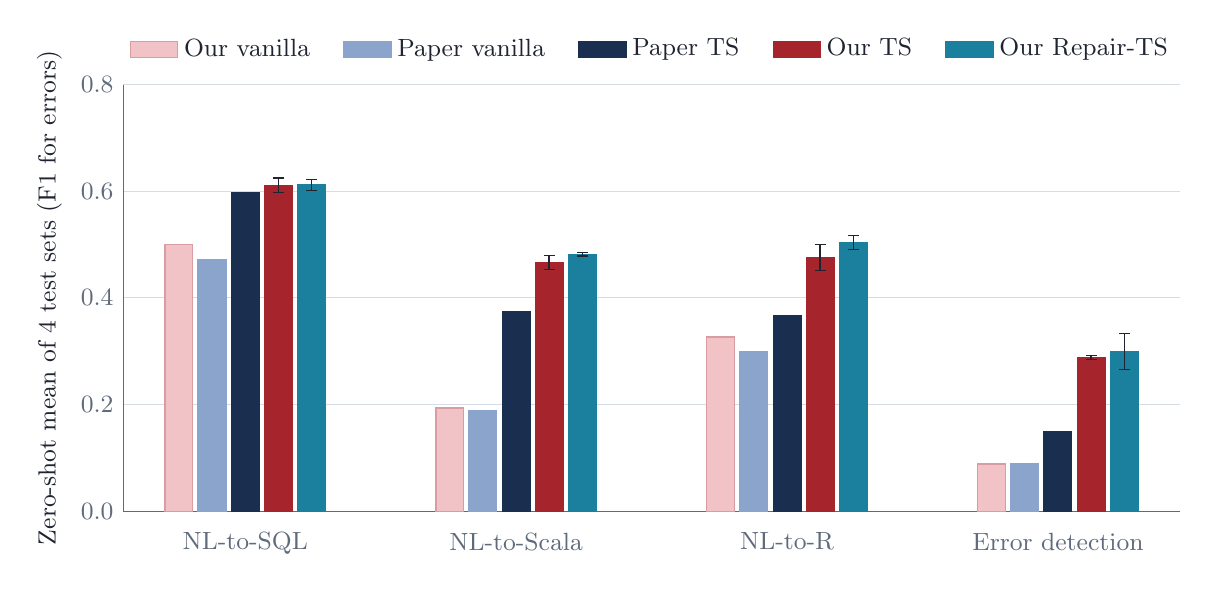
\begin{tikzpicture}
\begin{axis}[rd, ybar, bar width=10pt, width=15cm, height=7cm, ymin=0, ymax=0.8,
  symbolic x coords={NL-to-SQL,NL-to-Scala,NL-to-R,Error detection}, xtick=data, enlarge x limits=0.15,
  ylabel={Zero-shot mean of 4 test sets (F1 for errors)}, ytick={0,0.2,...,0.8}, y tick label style={/pgf/number format/.cd,fixed,fixed zerofill,precision=1},
  error bars/error bar style={tsink,line width=0.6pt}, error bars/error mark options={rotate=90,mark size=2pt,tsink},
  legend style={at={(0.5,1.03)},anchor=south,legend columns=5}]
\addplot[area legend,fill=cVanOurs,draw=tsred!45] coordinates {(NL-to-SQL,0.5001) (NL-to-Scala,0.1936) (NL-to-R,0.3267) (Error detection,0.0885)};
\addplot[area legend,fill=cVanPaper,draw=cVanPaper] coordinates {(NL-to-SQL,0.4708) (NL-to-Scala,0.1878) (NL-to-R,0.2993) (Error detection,0.0895)};
\addplot[area legend,fill=tsnavy,draw=tsnavy] coordinates {(NL-to-SQL,0.5982) (NL-to-Scala,0.3750) (NL-to-R,0.3658) (Error detection,0.1485)};
\addplot[area legend,fill=tsred,draw=tsred,error bars/.cd,y dir=both,y explicit] coordinates {(NL-to-SQL,0.6113) +- (0,0.0135) (NL-to-Scala,0.4666) +- (0,0.0129) (NL-to-R,0.4760) +- (0,0.0242) (Error detection,0.2882) +- (0,0.0042)};
\addplot[area legend,fill=cRepair,draw=cRepair,error bars/.cd,y dir=both,y explicit] coordinates {(NL-to-SQL,0.6122) +- (0,0.0107) (NL-to-Scala,0.4817) +- (0,0.0031) (NL-to-R,0.5043) +- (0,0.0128) (Error detection,0.2992) +- (0,0.0335)};
\legend{Our vanilla,Paper vanilla,Paper TS,Our TS,Our Repair-TS}
\end{axis}
\end{tikzpicture}
\end{document}
